\documentclass[conference]{IEEEtran}
\usepackage[hidelinks]{hyperref}
\usepackage{amsmath,amsfonts}
\usepackage{algorithmic}
\usepackage{graphicx}
\usepackage{placeins}
\usepackage{url}
\usepackage{algorithm}

\begin{document}

\title{Summer'26 Report: Algorithm Unrolling}

\author{\IEEEauthorblockN{Sai Ritvik Uppuganti [2025122012]}
\IEEEauthorblockA{\textit{Signal Processing and Communications Research Center (SPCRC)} \\
\textit{IIIT Hyderabad}\\}}

\maketitle

\begin{abstract}
This report explores algorithm unrolling, a framework that bridges iterative signal processing and deep neural networks by mapping optimization steps directly to network layers. We first analyze LISTA's mechanics and prerequisites, then connect these principles to modern white-box transformers (CRATE). Building on this foundation, we explore broader unrolled applications (Monga et al.) and connect these classical principles to modern white-box transformers like CRATE and CRATE-$\alpha$. The report ends with a PyTorch implementation of a 16-layer LISTA baseline on synthetic sparse-recovery data. This baseline successfully matched classical ISTA's accuracy with a 5 to 17$\times$ reduction in required iterations, establishing the training pipeline for future research directions.
\end{abstract}

\section{Introduction}
% Discuss the gap between classical iterative methods and black-box DNNs.

\subsection{Learning to Optimize (CVPR 2022) \texorpdfstring{\cite{chen2021learning}}{}}

In traditional machine learning (ML), the process is akin to \textit{induction}: learning from problems and answers, much like using flashcards. Optimization, on the other hand, is \textit{prescriptive}. It relies on problems and evaluations, similar to trying different routes to work every day and tracking commute times until the single fastest path is discovered. 

Classic optimization algorithms are hand-built on theory and experience, leaving practitioners to simply pick the algorithm. In Learning to Optimize (L2O), experts propose templates and training procedures. Practitioners then select a template and prepare the training data, thereby creating a trained algorithm for future use. Optimization algorithms are structurally similar to neural network (NN) layers:
\begin{itemize}
    \item \textit{Optimization Algorithm:} $x^{k+1} = \text{nonlin}(\text{lin}(x^{k})+\text{offset})$
    \item \textit{Single NN Layer:} $x^{k+1} = \text{ReLU}(\text{weights}(x^{k})+\text{bias})$
\end{itemize}
The only major difference is that in NNs (excluding RNNs), the nonlinear functions, linear functions, and offsets change significantly with each iteration $k$. Therefore, an optimization algorithm behaves similarly to an RNN. By taking a classic algorithm and unrolling its iterations into a finite NN, we untie the parameters. This allows the model to learn optimal, distinct weights for each layer, rather than being mathematically forced to remain identical at every step. The result is a solver that's slow to train but fast at inference — the opposite trade-off from classic ISTA.

There are two main neural network architectures for optimization:
\begin{enumerate}
    \item \textit{Model-Free (Black-Box):} Like traditional deep learning, this approach takes inputs, trains, and gives outputs while ignoring the mathematical structure of optimization.
    \begin{itemize}
        \item \textit{Pros:} Extremely fast inference due to having very few layers.
        \item \textit{Cons:} Massive number of parameters, very slow training, and poor generalization.
    \end{itemize}
    \item \textit{Model-Based (White/Gray-Box):} This starts with an optimization algorithm and neuralizes it. Deep learning is applied to specific parts of the algorithm that need acceleration or flexibility.
\end{enumerate}

The model-based approaches include three main types:
\begin{itemize}
    \item \textit{Algorithm Unrolling (AU):} Maps classic iterative algorithm steps into NN layers.
    \item \textit{Plug-and-Play (PnP):} Replaces one specific math step in a classic algorithm (often the prior or regularization step) with a pre-trained NN, such as an image denoiser.
    \item \textit{Deep Equilibrium Models (DEQ):} Designs a network to find a fixed point or equilibrium state for convergence.
\end{itemize}

\subsubsection{Algorithm Unrolling (AU) and LASSO \texorpdfstring{\cite{monga2021algorithm}}{}}

Algorithm unrolling involves two key steps: picking a classic iteration to unroll into an NN, and selecting a set of NN parameters to learn.

Consider the LASSO example:
\begin{equation}
x^{\text{lasso}} \leftarrow \arg\min_x \frac{1}{2}\|Ax-b\|_2^2 + \lambda\|x\|_1
\end{equation}
The goal is to recover $x^{\text{true}}$ from a noisy measurement $b = Ax^{\text{true}} + n$. The two terms pull in opposite directions:
\begin{itemize}
    \item \textit{Data Fidelity:} $\frac{1}{2}\|Ax-b\|_2^2$ ensures the guessed signal matches the physical measurements. Over-prioritizing this fits the messy noise, resulting in many non-zero values.
    \item \textit{Regularizer:} $\lambda\|x\|_1$ is a penalty that forces the solution to be sparse. Over-prioritizing this minimizes values to 0 to clean the signal, causing the predicted measurements to stop matching the raw data.
\end{itemize}

For an optimization problem, you generally evaluate the derivative and walk down the slope until it becomes exactly flat (derivative = $0$). The L2 norm ($y = x^2$) yields a smooth parabola, so gradient descent easily reaches $x=0$. However, the L1 norm ($y = |x|$) creates a sharp, V-shaped curve. The slope is $-1$ on the left and $1$ on the right, but it is entirely non-differentiable at $x=0$. Because gradient descent requires a derivative to find the step direction, and LASSO's goal is to force sparsity, the algorithm breaks down when it reaches $0$ because the derivative cannot be computed.

\subsubsection{Iterative Soft-Thresholding Algorithm (ISTA)}
ISTA handles this issue by separating the tasks. It uses standard smooth derivatives to handle the least-squares part of the equation, and it applies a separate, non-derivative mathematical rule (soft-thresholding) to forcibly handle the sharp, undefined corners of the L1 norm.

The ISTA update rule is:
\begin{equation}
x^{k+1} = \eta_{\lambda\alpha} (x^k - \alpha A^T (Ax^k - b))
\end{equation}
Here, the gradient descent step is $x^k - \alpha A^T(Ax^k - b)$, which minimizes the least-squares error. $\alpha$ is the step size required for convergence. Soft-thresholding, represented by $\eta_{\lambda\alpha}(\cdot)$, is applied element-wise to the gradient step's result. It mathematically shrinks small values toward zero to serve as a proxy for the sparsity constraint.

Note that $(Ax^k - b)$ is the error (predicted minus measured), and $A^T$ projects that error back into signal space. The initial guess is updated by subtracting a small fraction $\alpha$ of that error. The term $\lambda\alpha$ acts as the noise gate, and $\eta$ is the filter. If a value in the signal is below the gate, it goes to 0; if it is above the gate, it is slightly shrunk but remains.

\subsubsection{Learned ISTA (LISTA)}
Gregor and LeCun (2010) \cite{gregor2010learning} proposed freeing the parameters of ISTA. Starting with the known formula, we expand it to:
\begin{align}
x^{k+1} &= \eta_{\lambda\alpha} (x^k - \alpha A^T A x^k + \alpha A^T b) \\
x^{k+1} &= \eta_{\lambda\alpha} ((I - \alpha A^T A)x^k  + \alpha A^T b)
\end{align}
Let $W_1 = \alpha A^T$, $W_2 = I - \alpha A^T A$, and let $\theta = \lambda\alpha$ (the threshold). This simplifies to:
\begin{equation}
x^{k+1} = \eta_\theta(W_1 b + W_2 x^k)
\end{equation}

\begin{algorithm}[htbp]
\caption{Forward Pass of the Unrolled LISTA Network}
\label{alg:lista}
\begin{algorithmic}[1]
\REQUIRE Measurement $b$, Iterations $K$, Learned Weights $\{W_1^k, W_2^k\}_{k=1}^K$, Thresholds $\{\theta^k\}_{k=1}^K$
\STATE \textbf{Initialize:} $x^0 = \mathbf{0}$
\FOR{$k = 1$ to $K$}
    \STATE $c^k = W_1^k b + W_2^k x^{k-1}$
    \STATE $x^k = \text{sgn}(c^k) \max(|c^k| - \theta^k, 0)$
\ENDFOR
\RETURN $x^K$
\end{algorithmic}
\end{algorithm}


\begin{figure}[htbp]
\centering
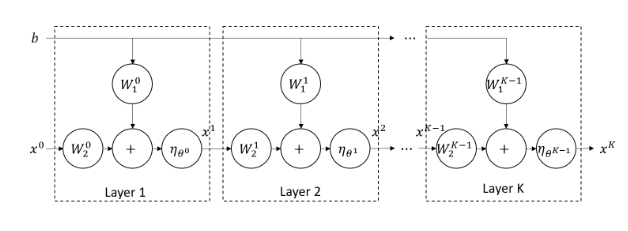
\includegraphics[width=\columnwidth]{attachments/lista_architecture.png}
\caption{LISTA network architecture unrolled over $K$ layers.}
\label{fig:lista_arch}
\end{figure}

This is structurally identical to a standard Recurrent Neural Network (RNN) or residual network layer, but with untied parameters. Here, $W_2 x^k$ is the linear weight matrix multiplied by the hidden state from the previous layer, and $W_1 b$ is the linear projection of the input data (acting as a bias added at every step). Finally, $\eta_\theta$ serves as a non-linear activation function comparable to ReLU. 

Because the parameters are free and learnable for every layer, inference is much faster, while the physical matrix $A$ remains fixed. 

ISTA requires very small steps to guarantee mathematical convergence because it is a general-purpose algorithm. The step size $\alpha$ must be strictly bounded by the maximum eigenvalue (the inverse of the Lipschitz constant) of the matrix $A^T A$. If it steps any larger, it might overshoot the minimum and explode ($\alpha < 2/L$, where $L = \lambda_{\max}(A^T A)$).

LISTA training takes time, but its inference is instantaneous. Because it is based on a specific dataset, it takes shortcuts from the statistics it learned:
\begin{itemize}
    \item \textit{Preconditioning:} The geometry of the data fidelity term is dictated entirely by its Hessian matrix. The condition number $\kappa$ of the Hessian matrix $A^T A$ is $\lambda_{\max}(A^T A)/\lambda_{\min}(A^T A)$. When $\kappa = 1$, all eigenvalues are equal, making the objective function's contour lines perfect bowl-shaped hyperspheres where the negative gradient points directly at the global minimum. When $\kappa \gg 1$, the matrix is ill-conditioned, stretching the contour lines into skewed ellipses. This forces the gradient to zig-zag to reach convergence. LISTA unties the weights to learn $W_2$, which acts as a learned preconditioner. It actively modifies the iteration matrix's eigenspectrum to cluster the effective Hessian's eigenvalues closer to 1, suppressing extreme values and allowing the level sets to become closer to hyperspheres.
    \item \textit{Exploiting the Prior:} ISTA relies on a generic L1 prior, forcing it to start completely blind at $x^0=0$ for every new data point. LISTA replaces this assumption with the dataset's probability distribution. By retaining memory of previous training pairs, the first unrolled layer acts as a data-driven projection matrix. When computing $x_1 = \eta_\theta(W_1 b)$, $W_1$ instantly correlates the new measurement $b$ against learned patterns of how the system's physics corrupts the signal. This projects the initial guess directly onto the true data manifold, bypassing the need to search from zero and drastically reducing required convergence steps.
\end{itemize}

\begin{figure}[htbp]
\centering
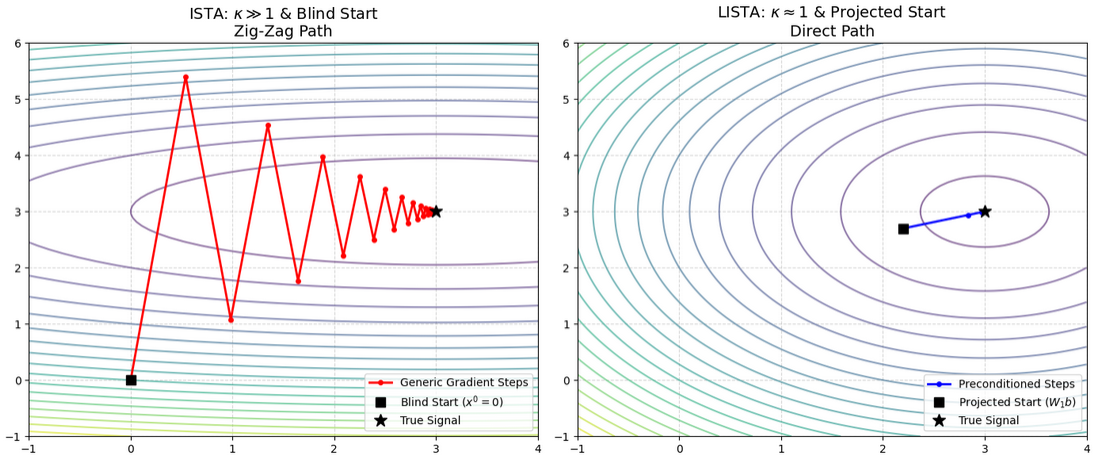
\includegraphics[width=\columnwidth]{attachments/ista_vs_lista.png}
\caption{Convergence paths: Zig-zag (ISTA) vs. Direct (LISTA).}
\label{fig:convergence_path}
\end{figure}

Training LISTA involves three steps:
\begin{enumerate}
    \item \textit{Generating the Dataset:} Fix a random measurement matrix $A$. Artificially generate thousands of sparse ground truth signals ($x^{\text{true}}$) with varying random spikes. Multiply by $A$ and add simulated noise to get observed measurements $b$, forming supervised training pairs: $(x^{\text{true}}, b)$.
    \item \textit{Forward Pass and Loss:} Fix a small $K$ (e.g., $K=16$ layers). Feed a batch of $b$ through the layers to get a final prediction $x^K(b)$. The loss function is the standard L2 norm (MSE) comparing the output with the ground truth.
    \item \textit{Back-propagation:} Apply Stochastic Gradient Descent (SGD) to minimize the L2 loss: $\sum \|x^K(b) - x^{\text{true}}\|_2^2$. Update the free parameters ($\theta^k, W_1^k, W_2^k$) for every layer to minimize loss.
\end{enumerate}

Neural networks handle the sharp non-differentiable corner of soft-thresholding using subgradients. For the function $\eta_\theta(x) = \text{sgn}(x)\max(|x|-\theta, 0)$:
\begin{itemize}
    \item If $|x| > \theta$, the gradient is $1$.
    \item If $|x| < \theta$, the gradient is $0$.
    \item If $|x| = \theta$, the derivative doesn't exist, but frameworks like PyTorch assign a valid subgradient (usually $0$ or $1$) at that exact point. The probability of a floating-point value landing exactly on $\theta$ is effectively zero, preventing disrupted gradient flow.
\end{itemize}
The trained network reaches ISTA's accuracy in roughly 50$\times$ fewer iterations — and lands at a lower final error, because it was trained directly against $x^{\text{true}}$ rather than searching from scratch.

\begin{figure}[htbp]
\centering
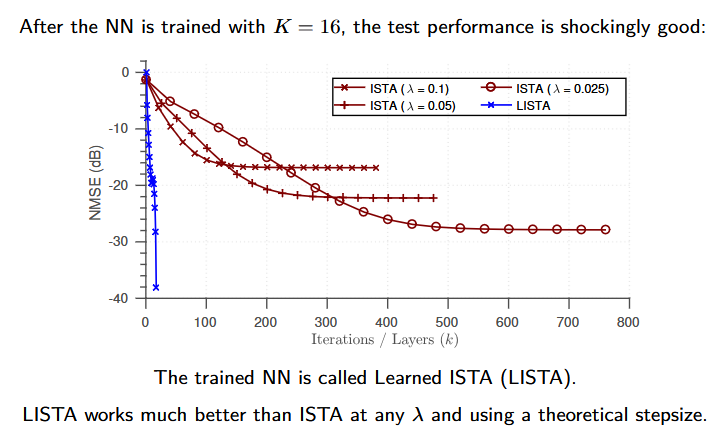
\includegraphics[width=\columnwidth]{attachments/nmse_vs_iterations.png}
\caption{Performance comparison: NMSE (dB) vs Iterations/Layers.}
\label{fig:nmse_plot}
\end{figure}

\begin{table}[htbp]
\caption{Comparison: Traditional Neural Network vs. Algorithm Unrolling (LISTA)}
\centering
\begin{tabular}{|p{1.5cm}|p{2.3cm}|p{2.4cm}|}
\hline
\textbf{Aspect} & \textbf{Traditional NN} & \textbf{Algorithm Unrolling} \\ \hline
Training Code / Loop & PyTorch / SGD / Backprop & PyTorch / SGD / Backprop \\ \hline
Data Source & Collected real-world datasets & Synthesized via matrix $A$ \\ \hline
Hidden Layer Sizes & Arbitrary hyperparameter & Locked to dimensions of $A$ \\ \hline
Activation Function & General (ReLU, GELU) & Optimization proxy (Soft-Thresholding) \\ \hline
What Layers Mean & Abstract feature hierarchies & Successive iterations of math solver \\ \hline
\end{tabular}
\label{tab:comparison}
\end{table}


\subsubsection{Applications and Challenges}
Algorithm unrolling extends naturally to other operator-splitting methods like ADMM and PDHG. Key applications:
\begin{itemize}
    \item \textit{CT Reconstruction:} Using $b = Ax + \text{noise}$ (where $A$ is the Radon transform), AU yields cleaner images than classic Total Variation (TV) methods or pure black-box CNNs.
\end{itemize}

\begin{figure}[htbp]
\centering
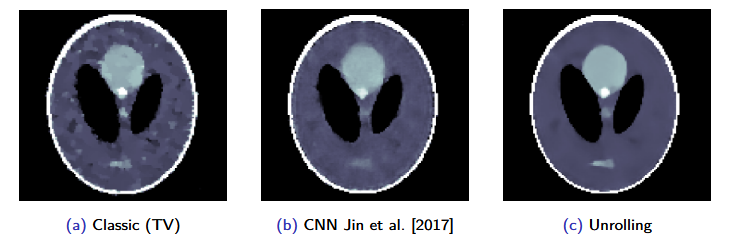
\includegraphics[width=\columnwidth]{attachments/ct_recon.png}
\caption{CT Reconstruction results: Classic TV vs CNN vs Unrolling.}
\label{fig:ct_recon}
\end{figure}

\begin{itemize}
    \item \textit{Image De-blurring:} Using $b = k * x + \text{noise}$ (where $k$ is an unknown blurring kernel), AU successfully recovers the kernel to create sharper images with less distortion.
\end{itemize}

\begin{figure}[htbp]
\centering
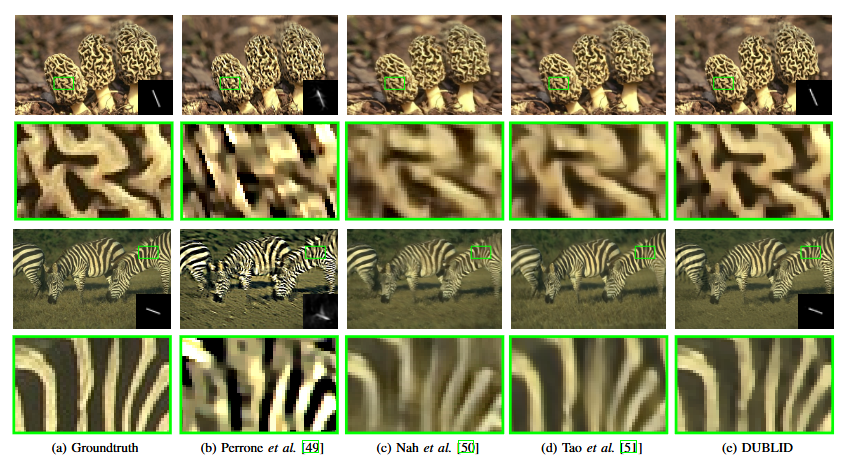
\includegraphics[width=\columnwidth]{attachments/deblur.png}
\caption{Image Deblurring results: Total Variation vs CNN vs Unrolling.}
\label{fig:deblurring}
\end{figure}

However, AU presents several challenges:
\begin{itemize}
    \item \textit{Parameter Overhead:} Learning distinct weights for every layer demands $\mathcal{O}(n^2K + mnK)$ parameters, making training very slow. This forces a trade-off when selecting $K$: too small results in poor convergence, and too large causes exploding or vanishing gradients.
    \item \textit{Interpretability:} Critical fields like medical imaging require white-box explainability, but AU parameters are still inherently black-box.
    \item \textit{Generalizability:} If given out-of-distribution data, the solver should not fail terribly; its worst-case performance must at least match the classic math algorithm to retain reliability.
\end{itemize}

\subsubsection{Advances in LISTA}
Subsequent work addressed these directly:
\begin{itemize}
    \item \textit{LISTA-CP (Weight Coupling) \cite{chen2018theoretical}:} Theoretical analysis showed that as iterations $k \to \infty$, $W_2^k + W_1^k A \to I$ and the threshold $\theta^k \to 0$. Instead of letting the network learn this slowly, LISTA-CP enforces $W_2^k = I - W_1^k A$ from layer 1. This eliminates the need to learn $W_2$, drastically reducing free parameters to $\mathcal{O}(mnK)$ and making training highly stable. 
    \item \textit{LISTA-SS (Support Selection):} At each iteration, the largest signal spikes bypass soft-thresholding. Soft-thresholding kills noise but artificially shrinks true peaks. Bypassing these spikes eliminates shrinkage bias, accelerating the convergence rate and achieving a lower final reconstruction error.
    \item \textit{LISTA-CPSS:} Combining both CP and SS drastically improves convergence speed and the final normalized mean square error over standard LISTA.
\end{itemize}
\begin{figure*}[!t]
\centering
\begin{tabular}{cc}
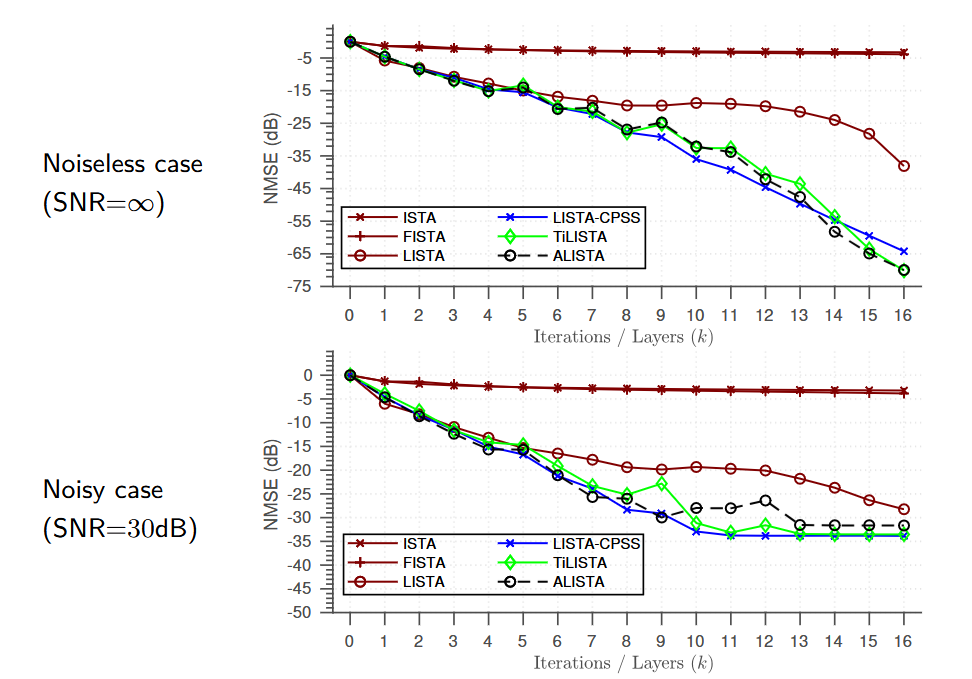
\includegraphics[width=0.43\textwidth]{attachments/snr.png} &
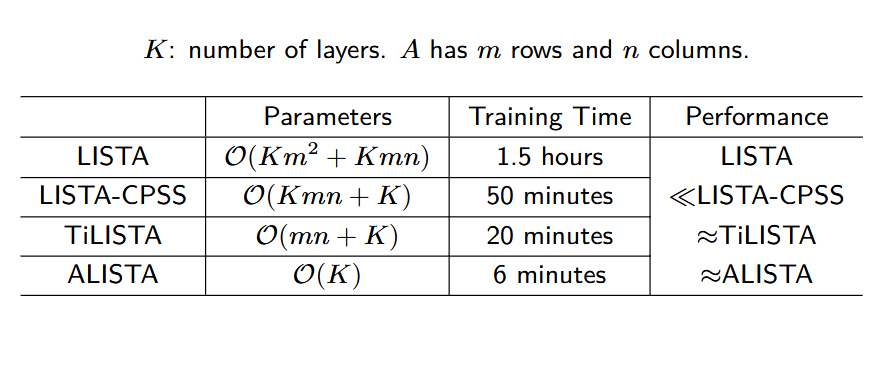
\includegraphics[width=0.43\textwidth]{attachments/complex.png} \\
(a) Noiseless ($\text{SNR}=\infty$) and Noisy ($\text{SNR}=30\text{dB}$) & (b) Complexity \& training time table \\[6pt]
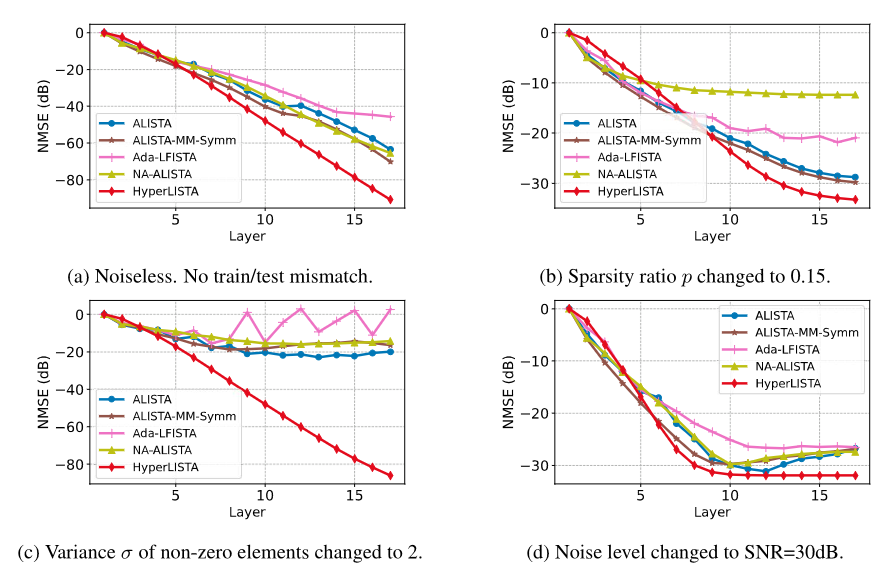
\includegraphics[width=0.43\textwidth]{attachments/nmse.png} &
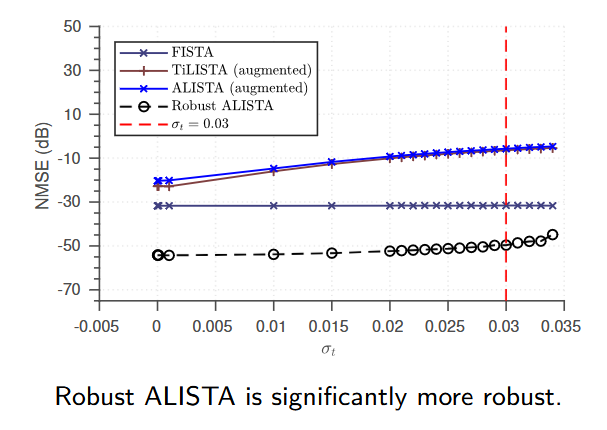
\includegraphics[width=0.43\textwidth]{attachments/rob.png} \\
(c) Robust ALISTA vs. noise levels & (d) Robustness across sparsity \& variance \\
\end{tabular}
\caption{Performance and robustness evaluations across advanced LISTA variants.}
\label{fig:advanced_lista_grid}
\end{figure*}

Other prominent advances include TiLISTA (tied weights), ALISTA (analytic LISTA) \cite{liu2019alista}, Robust LISTA, ada-LISTA, and HyperLISTA.

\subsection{Fast Approximations of Sparse Coding (Gregor and LeCun, 2010) \texorpdfstring{\cite{gregor2010learning}}{}}

In Sparse Coding (SC), input vectors are reconstructed using a sparse linear combination of basis vectors. SC has become a popular method for extracting features from data. For a given input, SC minimizes a quadratic reconstruction error combined with an L1 penalty term on the code. However, this iterative process is often too slow for applications such as real-time pattern recognition. 

To address this, the authors proposed two versions of a very fast algorithm that produces approximate estimates of the sparse code. These estimates can be used to compute good visual features or to initialize exact iterative algorithms. The core idea is to train a non-linear, feed-forward predictor with a specific architecture and a fixed depth to produce the best possible approximation of the sparse code. 

A specific version of this method, which functions as a trainable iteration of Li and Osher’s coordinate descent method, produces approximate solutions with 10 times less computation than Li and Osher’s approach for the exact same approximation error. Unlike earlier proposals for sparse code predictors, this system allows a form of approximate ``explaining away'' to take place during inference. Furthermore, the resulting predictor is entirely differentiable, allowing it to be seamlessly integrated into globally-trained recognition systems.

Table \ref{tab:sc_vs_lasso} maps Gregor and LeCun's Sparse Coding (SC) terminology to the standard LASSO formulation.

\begin{table}[htbp]
\caption{Terminology Mapping: Sparse Coding vs. LASSO}
\centering
\begin{tabular}{|l|l|}
\hline
\multicolumn{1}{|c|}{\textit{Sparse Coding}} & \multicolumn{1}{c|}{\textit{LASSO (Sparse Signal Recovery)}} \\ \hline
Dictionary matrix ($W_d$) & Measurement matrix ($A$) \\ \hline
Input vector ($X$) & Observed measurement ($b$) \\ \hline
Sparse code vector ($Z$) & True signal ($x^{\text{true}}$) \\ \hline
Filter matrix ($W_e$) & Feed-forward projection matrix ($W_1$) \\ \hline
Mutual inhibition matrix ($S$) & Recurrent/hidden state matrix ($W_2$) \\ \hline
Shrinkage function ($h_\theta$) & Soft-thresholding operator ($\eta_\theta$) \\ \hline
\end{tabular}
\label{tab:sc_vs_lasso}
\end{table}

\subsection{Model-Based Deep Learning for Sensing and Imaging (Eldar, 2023) \texorpdfstring{\cite{shlezinger2023model}}{}}

Yonina Eldar's work on model-based deep learning and biomedical image reconstruction shows that combining classical optimization with deep learning creates efficient, interpretable models. Through various publications and lectures, several critical insights regarding algorithm unrolling and its theoretical boundaries were established.

\subsubsection{Architecture and Training Methodologies}
\begin{itemize}
    \item \textit{Source of Training Data:} The physical mathematical model is utilized in multiple ways. It dictates the network architecture itself, and its equations can be embedded directly into the training metric. This enables the model to effectively generate its own training data, meaning external supervised datasets are not strictly required.
    \item \textit{Comparison to PINNs:} Physics-Informed Neural Networks (PINNs) incorporate physics solely within the loss function. In contrast, the true power of algorithm unrolling lies in utilizing physics to construct the actual architecture of the neural model.
    \item \textit{Optimization Loss vs. Machine Learning Metric:} There are fundamentally two distinct loss mechanisms. The optimization loss determines the network's structural architecture. The external learning metric trains the network's parameters. If the optimization metric is used as the loss function, the network can be trained entirely without supervision. If labeled data is available, this metric can simply be combined with a standard supervised loss.
    \item \textit{Tied vs. Untied Layers:} Unrolled layers can feature tied parameters (fixed across all layers) or untied parameters (distinct for each layer). As a general rule, \textit{untied} layers are preferred because they provide significantly more expressive power. However, \textit{tied} layers are beneficial when the training dataset is very small (thereby reducing the number of learnable parameters) or when the underlying layers represent a physical property that must remain uniform, such as estimating an unknown communication channel.
    \item \textit{Freed Parameters in Complex Models:} In highly complex real-world applications like ultrasound—where assuming human tissue is strictly low-rank and sparse is an overly simplistic model—all parameters can be freed. Because the unrolled network is intentionally shallow (e.g., unrolled to only about 10 layers), the total parameter count remains highly manageable even when everything is freed.
\end{itemize}

\subsubsection{Theoretical Bounds and Convergence}
\begin{itemize}
    \item \textit{Parameter Convergence Across Layers:} It is tempting to assume that the learned parameters across layers simply converge to the mathematical ideals of the classic algorithm. However, an unrolled network solving a problem in 10 iterations cannot simply be a ``faster ISTA,'' as ISTA typically requires roughly 20,000 iterations to reach mathematical convergence. Instead, the learned parameters converge to something completely different, taking a highly accelerated, alternative optimization path.
    \item \textit{Cheating Optimization Bounds:} Unrolled networks often appear to beat established mathematical optimization bounds. This occurs because the model mathematically ``cheats'' by leveraging training data. Classic bounds were formulated without the assumption of data-driven priors, whereas unrolled networks use this training data to aggressively guide the solver to a better local minimum much faster.
    \item \textit{Lipschitz Bounds and Generalization:} For these structured, model-based networks, the generalization error decays exponentially with the depth (number of layers). It can be formally proven that, assuming the soft-thresholding parameter is chosen appropriately, the generalization bound of an unrolled network is always smaller than the bound of an equivalent unstructured standard network. 
    \item \textit{Dimensionality:} A major advantage of this model-based approach is its inherent insensitivity to the dimensionality of the specific problem being solved.
    \item \textit{Learning Biases \& Estimation Theory:} While algorithm unfolding is a highly generic approach, there are special cases—such as formalizing a Gaussian model—where direct mathematical equivalences to classical estimation theory can be established.
\end{itemize}

\subsection{Comparative Analysis with Sister Architectures}

Algorithm unrolling maps steps to finite layers. Alternative approaches, such as Plug-and-Play (PnP) priors and Deep Equilibrium (DEQ) models, tackle this intersection differently:

\subsubsection{Plug-and-Play (PnP) Priors \texorpdfstring{\cite{venkatakrishnan2013plug}}{}}

The Plug-and-Play approach modifies a classic optimization algorithm by replacing one specific mathematical step—typically the prior or regularization step—with a pre-trained neural network, such as an advanced image denoiser. 

It utilizes the Alternating Direction Method of Multipliers (ADMM) technique to decouple the overarching problem into two distinct steps:
\begin{itemize}
    \item \textit{Step 1 (Forward Model):} Handles the physics and empirical measurements.
    \item \textit{Step 2 (Prior Model):} Handles the denoising and regularization.
\end{itemize}

The core optimization problem is formulated as:
\begin{equation}
\min f(x) + g(z) \quad \text{subject to} \quad Ax + Bz = c
\end{equation}

The ``plug-and-play'' element involves swapping out the prior model step entirely in favor of a state-of-the-art neural network, without altering the rest of the mathematical framework. 

\textit{Advantage:} PnP keeps the classical infinite optimization loop and its convergence guarantees intact, while plugging deep learning in only where it matters — the denoising step.

\subsubsection{Deep Equilibrium Models (DEQ) \texorpdfstring{\cite{bai2019deep}}{}}

Rather than unrolling an algorithm for a fixed number of iterations, Deep Equilibrium Models design the network to find a fixed point (an equilibrium state) that dictates convergence.

\textit{Working Mechanism:} Standard algorithm unrolling dictates unfolding the process for $K$ layers and tracking the data sequentially, layer-by-layer. DEQ, however, unrolls a weight-tied network to infinity ($k \to \infty$). Because an infinite-depth neural network eventually hits a stable equilibrium state, DEQ skips the layer-by-layer math entirely. Instead, it utilizes a root-finding algorithm to jump straight to the fixed point.

\textit{Advantage (Resolving the Memory Bottleneck):} Standard unrolling must store intermediate states across all $K$ layers for backpropagation — a significant memory cost. DEQ sidesteps this by jumping to the fixed point and using implicit differentiation to backpropagate analytically, training an ``infinite-depth'' network at $\mathcal{O}(1)$ memory.

\subsection{Algorithm Unrolling: Applications and Extensions (Monga et al.) \texorpdfstring{\cite{monga2021algorithm}}{}}

Vishal Monga et al.'s survey maps how algorithm unrolling applies across different domains. Most of this reporting period's depth went into ISTA/LISTA itself (Section~I.A); the following applications are covered at survey level — sufficient to map each domain's classic algorithm onto its unrolled architecture, but not to the same derivational depth as the LISTA section — and are included to establish breadth of the design space before the next phase narrows to one target application.
\subsubsection{Learned ISTA (LISTA) and Overcomplete Dictionaries}
In the context of sparse coding, an overcomplete dictionary $W \in \mathbb{R}^{n \times m}$ has $n$ rows (representing the dimension of the signal) and $m$ columns (the number of building blocks), where $m > n$. Because this dictionary contains redundant columns, there are theoretically an infinite number of mathematical combinations to approximate the signal $y$. Sparse coding algorithms like ISTA exploit this redundancy by searching for the one specific combination that utilizes the absolute fewest columns possible to approximate $y$. 

When unrolled, the network is trained via loss minimization using gradient-based learning techniques, such as Stochastic Gradient Descent (SGD). The loss function is formulated as:
\begin{equation}
\ell(W_t, W_e, \lambda) = \frac{1}{N} \sum_{n=1}^{N} \| \hat{x}^n(y^n; W_t, W_e, \lambda) - x^{*n} \|_2^2
\end{equation}
In this framework, the weights effectively act as the measurement matrix, optimizing the sparse recovery process.

\subsubsection{DUBLID: Blind Image Deblurring}
A spatially invariant blurring process can be represented as a discrete convolution:
\begin{equation}
y = k * x + n
\end{equation}
where $y$ is the blurred image, $x$ is the latent sharp image, $k$ is the unknown blur kernel, and $n$ is Gaussian random noise. Because natural images usually feature flat regions separated by sharp edges, their gradients (derivatives) are highly sparse. Total Variation (TV) minimization leverages this prior by attempting to find the kernel $k$ and the image gradients ($g_1, g_2$) that best explain the blurred image $y$, while forcing the gradients to be sparse:
\begin{equation}
\begin{aligned}
\min_{k,g_1,g_2} &\frac{1}{2}(\|D_x y - k * g_1\|_2^2 + \|D_y y - k * g_2\|_2^2) \\
&+ \lambda_1\|g_1\|_1 + \lambda_2\|g_2\|_1 + \frac{\epsilon}{2}\|k\|_2^2
\end{aligned}
\end{equation}
subject to $\|k\|_1 = 1, k \ge 0$. 

A more robust, generalized version utilizes a set of $C$ different linear filters ($f_i$) to extract gradient features rather than relying solely on basic horizontal and vertical derivatives:
\begin{equation}
\min_{k,\{g_i\}_{i=1}^C} \sum_{i=1}^C \left( \frac{1}{2}\|f_i * y - k * g_i\|_2^2 + \lambda_i\|g_i\|_1 \right) + \frac{\epsilon}{2}\|k\|_2^2
\end{equation}
Because these variables are heavily coupled and computationally brutal to solve simultaneously, the Half-Quadratic Splitting (HQS) algorithm is utilized. HQS introduces auxiliary variables ($z_i$) to split the overarching equation into a sequence of simpler, decoupled sub-problems:
\begin{equation}
\begin{aligned}
\min_{k,\{g_i,z_i\}_{i=1}^C} \sum_{i=1}^C \bigg( &\frac{1}{2}\|f_i * y - k * g_i\|_2^2 + \lambda_i\|z_i\|_1 \\
&+ \frac{1}{2\zeta_i}\|g_i - z_i\|_2^2 \bigg) + \frac{\epsilon}{2}\|k\|_2^2
\end{aligned}
\end{equation}
A new penalty parameter, $\zeta_i$, penalizes the difference between the true gradient $g_i$ and the auxiliary variable $z_i$. As $\zeta_i$ increases, $g_i$ and $z_i$ are mathematically forced to become identical.

This sequential decoupling provides a clean, closed-form analytical solution for each variable, allowing the process to be seamlessly cast into network layers:
\begin{itemize}
    \item \textit{Updating $g_i$:} Involves spatial domain convolutions, which are slow. This is resolved by computing the Fast Fourier Transform (FFT) and taking the inverse:
    \begin{equation}
    g_i^{l+1} = \mathcal{F}^{-1} \left\{ \frac{\zeta_i^l \hat{k}^{l*} \odot \hat{f}_i^{l*} \odot \hat{y} + \hat{z}_i^l}{\zeta_i^l |\hat{k}^l|^2 + 1} \right\}
    \end{equation}
    \item \textit{Updating $z_i$:} Solved via a soft-thresholding operation, identical to ISTA:
    \begin{equation}
    z_i^{l+1} = \mathcal{S}_{\lambda_i^l / \zeta_i^l}\{g_i^{l+1}\}
    \end{equation}
    \item \textit{Updating $k$:} Utilizes FFT for speed, applies a ReLU operator ($[\cdot]_+$) to ensure kernel values do not go negative, and uses a normalization operator ($\mathcal{N}_1$) to ensure the kernel sums to 1 for energy conservation:
    \begin{equation}
    k^{l+1} = \mathcal{N}_1 \left[ \mathcal{F}^{-1} \left\{ \frac{\sum_{i=1}^C \hat{z}_i^{l+1*} \odot \hat{f}_i^{l*} \odot \hat{y}}{\sum_{i=1}^C |\hat{z}_i^{l+1}|^2 + \epsilon} \right\} \right]_+
    \end{equation}
\end{itemize}

In the unrolled architecture, the parameters $\zeta, \beta, f$ become learnable weights. Refined estimates for the image gradients and the blur kernel are obtained after $L$ iterations, and the final image is retrieved by solving a least-squares problem where the filter coefficients are shared with the intermediate layer updates. The entire pipeline is updated jointly using a translation-invariant mean-square-error loss to compensate for possible spatial shifts.

\subsubsection{ADMM-CSNet: Compressive Sensing}
In compressive sensing, the goal is to rebuild an original signal $x$ from compressed measurements $y$. A linear filter $D_i$ (similar to a wavelet transform) is applied to make the signal sparse. By introducing a new auxiliary variable $z_i$ and forcing it to equal $D_i x$, the unrolled ADMM algorithm utilizes the Augmented Lagrangian:
\begin{equation}
\begin{aligned}
\mathcal{L}_\rho(x, z, \alpha) &= \frac{1}{2}\|\Phi x - y\|_2^2 + \sum_{i=1}^C \lambda_i g(z_i) \\
&+ \frac{\rho_i}{2}\|D_i x - z_i + \alpha_i\|_2^2
\end{aligned}
\end{equation}

Unlike HQS, ADMM introduces dual variables ($\alpha_i$) that act as an accumulator, tracking the constraint violation over time to force exact convergence. The iteration unrolls into three distinct updates:
\begin{itemize}
    \item \textit{Updating $x$:} A linear solver aggregates current guesses and performs matrix inversion to find the best signal fit.
    \item \textit{Updating $z$:} A non-linear step utilizes a proximal mapping operator to enforce sparsity.
    \item \textit{Updating $\alpha$:} A simple gradient ascent updates the dual variable based on the current error $(D_i x^l - z_i^l)$.
\end{itemize}
Unlike traditional ADMM, the unrolled network eliminates the need to manually guess penalty coefficients ($\rho$), step sizes ($\eta$), and regularization weights ($\lambda$) by learning them dynamically alongside the transform matrices $D_i$.

\subsubsection{CORONA: Ultrasound Clutter Suppression}
Ultrasound imaging captures frames containing echoes from static tissue and moving blood. The data matrix $D$ is modeled as $D = H_1 L + H_2 S + N$, where $L$ represents highly correlated, low-rank tissue signals and $S$ represents highly sparse blood vessel echoes. 

The optimization problem extracts $S$ and filters out $L$:
\begin{equation}
\min_{L,S} \frac{1}{2}\|D - (H_1 L + H_2 S)\|_F^2 + \lambda_1\|L\|_* + \lambda_2\|S\|_{1,2}
\end{equation}
The nuclear norm ($\|L\|_*$) promotes low-rank solutions for the static tissue, while the mixed $L_{1,2}$ norm ($\|S\|_{1,2}$) enforces row-wise sparsity for the blood signal. 

Running iterative SVDs and massive matrix multiplications on high-resolution frames is computationally prohibitive. CORONA unrolls this process into a CNN by replacing fixed matrices ($H_1, H_2$) with small, learnable convolution filters ($P_1^l$ through $P_6^l$):
\begin{align}
L^{l+1} &= \mathcal{T}_{\lambda_1^l}\{P_5^l * L^l + P_3^l * S^l + P_1^l * D\} \\
S^{l+1} &= \mathcal{S}_{\lambda_2^l}^{1,2}\{P_6^l * S^l + P_4^l * L^l + P_2^l * D\}
\end{align}
The network learns the optimal convolution filters and thresholding parameters layer-by-layer via backpropagation, utilizing ground truth matrices generated by the slow traditional algorithm to calculate the MSE loss.

\subsubsection{CRF-RNN: Semantic Segmentation}
Semantic segmentation requires classifying every single pixel to determine exact object boundaries. While standard deep neural networks simply guess a label, Conditional Random Fields (CRFs) assign labels based on a pixel's relationship with its neighbors. In Markov Random Fields, only pairwise interactions are considered.

Optimal labels are found by minimizing an energy function:
\begin{itemize}
    \item \textit{Unary Energy ($\phi_p$):} The raw, independent guess of a pixel's label based solely on image data, typically generated by a Fully Convolutional Network (FCN).
    \item \textit{Pairwise Energy ($\psi_{p,q}$):} A smoothness constraint penalizing mismatched labels on similar adjacent pixels to sharpen edges.
\end{itemize}

The Mean-Field (MF) algorithm solves these energy equations through four unrolled steps that map perfectly to network layers:
\begin{enumerate}
    \item \textit{Message Passing:} Compares pixel features using Gaussian kernels, acting exactly like a convolutional layer.
    \item \textit{Compatibility Transform:} Evaluates label compatibility, translating perfectly to a $1 \times 1$ convolution.
    \item \textit{Unary Addition:} Adds the original raw guess from the FCN back into the system via element-wise addition.
    \item \textit{Normalization:} Converts final scores into proper probabilities, functioning identically to a softmax layer.
\end{enumerate}
These steps map cleanly to network layers connected in a loop to form an RNN, allowing the FCN and CRF-RNN to be trained together end-to-end.

\begin{table*}[t!]
\caption{Comparative Overview of Unrolled Architectures}
\centering
\renewcommand{\arraystretch}{1.3}
\begin{tabular}{|p{2.5cm}|p{2.5cm}|p{2.5cm}|p{2.5cm}|p{2.5cm}|p{2.5cm}|}
\hline
\textbf{Network \& Application} & \textbf{Original Problem} & \textbf{Classic Iterative Algorithm} & \textbf{What Gets Unrolled \& Learnable} & \textbf{Physical Prior} & \textbf{Core Advantage} \\ \hline
\textbf{SCN (Single Image Super-Resolution)} & Recover a high-resolution image from a low-resolution observation. & Sparse Coding (LISTA) & Sparse coding iterations become layers. Dictionary atoms and mappings are learnable. & High-resolution patches admit sparse representations in a dictionary. & Faster, more accurate super-resolution; preserves edges and textures. \\ \hline
\textbf{DUBLID (Blind Image Deblurring)} & Recover both the sharp image and unknown blur kernel. & Half-Quadratic Splitting (HQS) & HQS stages become layers. Filters ($f_i$) and regularizations are learnable. & Natural images are piecewise smooth with sparse gradients. & $\sim 1000\times$ faster than classical TV blind deblurring with sharper reconstructions. \\ \hline
\textbf{ADMM-CSNet (Compressive Sensing)} & Reconstruct images from undersampled measurements. & ADMM & Variable-update steps become stages. Transforms ($D_i$) and penalties are learnable. & Variable splitting separates physics from image structure priors. & Comparable quality with less sampling and much faster reconstruction. \\ \hline
\textbf{CORONA (Ultrasound Clutter Suppression)} & Separate sparse blood flow signals from correlated tissue clutter. & Robust PCA / Matrix ISTA & Decomposition iterations become layers. Filters replace SVD matrix operations. & Tissue echoes are low-rank; blood signals are highly sparse. & Massive computational savings while preserving clutter suppression. \\ \hline
\textbf{CRF-RNN (Semantic Segmentation)} & Assign consistent semantic labels to image pixels. & Mean-Field Inference for CRFs & Message-passing iterations become recurrent layers. Compatibility transforms are learnable. & Nearby pixels with similar appearance should share labels. & Produces smoother, highly globally consistent image segmentations. \\ \hline
\textbf{Deep NMF (Source Separation)} & Separate mixed audio sources into interpretable components. & Non-negative Matrix Factorization & Multiplicative updates become layers. The basis dictionary ($W$) is learnable. & Spectral energy is non-negative; sources are sparse and additive. & Faster separation and better adaptation to real-world audio data. \\ \hline
\textbf{LISTA (Sparse Recovery)} & Recover sparse signals from corrupted measurements. & ISTA & Gradient and soft-thresholding iterations become layers. Weights and thresholds learnable. & Signals are sparse in a suitable representation. & Reaches mathematical accuracy in dramatically fewer iterations. \\ \hline
\end{tabular}
\label{tab:architecture_comparison}
\end{table*}


\subsubsection{Deep NMF: Source Separation}
Non-negative Matrix Factorization (NMF) decouples several audio signals from a mixture. The audio spectrogram is a massive matrix $M$ approximated as $M \approx WH$, where $W$ represents the fundamental spectral signatures and $H$ tracks the coefficients over time. Because physical audio energy is strictly positive, the algorithm enforces $W \ge 0$ and $H \ge 0$.

The cost function minimizes the difference between $M$ and $WH$ using the $\beta$-divergence ($D_\beta$) and an L1 penalty on $H$ for sparsity:
\begin{equation}
\min_{W \ge 0, H \ge 0} D_\beta(M | WH) + \mu\|H\|_1
\end{equation}
Because standard gradient descent subtracts values, potentially pushing matrices into negative numbers, multiplicative updates are utilized:
\begin{align}
H^l &= H^{l-1} \odot \frac{W^T [M \odot (WH^{l-1})^{\beta-2}]}{W^T (WH^{l-1})^{\beta-1} + \mu} \\
W^l &= W^{l-1} \odot \frac{[M \odot (W^{l-1}H^l)^{\beta-2}] {H^l}^T}{(W^{l-1}H^l)^{\beta-1} {H^l}^T}
\end{align}
Rather than forcing the network to calculate the massive update rule for $W$ in every single layer, Deep NMF completely unties $W$ from the iterative loop. $W$ becomes a set of standard trainable weights within the network, while only the $H$ update and normalization steps execute within the loops via backpropagation.



\subsubsection{Neural Network Training Using the Extended Kalman Filter (EKF)}
The Extended Kalman Filter (EKF) adapts to non-linear systems through iterative linearization. Because neural network training is a parameter estimation problem, the EKF can be directly applied where the ``state'' is the network weights ($w_k$) and the ``time step'' $k$ is the arrival of a new training sample:
\begin{align}
w_{k+1} &= w_k + \omega_k \\
y_k &= h_k(x_k; w_k) + \nu_k
\end{align}
Artificial process noise ($\omega_k$) prevents the mathematics from becoming overly confident and trapping the network in a local minimum.

The EKF linearizes the network using a first-order Taylor series expansion where the Jacobian ($H_k$) is calculated via standard backpropagation:
\begin{equation}
h_k(x_k; w_k) \approx h_k(x_k; \hat{w}_k) + H_k(w_k - \hat{w}_k)
\end{equation}
Instead of relying on a simple learning rate, the network executes three matrix multiplications to update weights:
\begin{align}
K_k &= P_k H_k (H_k^T P_k H_k + R_k)^{-1} \\
\hat{w}_{k+1} &= \hat{w}_k + K_k (y_k - \hat{y}_k) \\
P_{k+1} &= P_k - K_k H_k^T P_k + Q_k
\end{align}
The covariance matrix $P_k$ provides second-order derivative information regarding the curvature of the loss space, allowing massive, highly accurate steps that cut down required training epochs by orders of magnitude. 



\subsubsection{Convergence and Optimality Analysis of LISTA}
Analysis of the Iterative Hard Thresholding Algorithm (IHTA) provided theoretical clarity for LISTA. IHTA utilizes an L0 norm ($\|x\|_0 \le k$) to act as a hard limit on non-zero entries:
\begin{equation}
\min_x \frac{1}{2}\|y - Wx\|_2^2 \quad \text{subject to} \quad \|x\|_0 \le k
\end{equation}
The unrolled layer for this hard-thresholding setup is:
\begin{equation}
x^{l+1} = \mathcal{H}_k\{W_t x^l + W_e y\}
\end{equation}
Researchers proved that for an unrolled network to successfully recover a signal, the learned weight matrix must take the mathematical form $I - \Gamma W$:
\begin{equation}
W_t = I - \Gamma W
\end{equation}
Furthermore, as the network becomes incredibly deep ($l \to \infty$), the weights stop behaving randomly and achieve asymptotic weight coupling ($W_t^l - (I - W_e^l W) \to 0$). Forcing this coupling from the start allowed researchers to mathematically prove that the unrolled network achieves a linear convergence rate, establishing that pure-math analytical weights can perform just as efficiently as deep learning models trained on GPUs.



\section{Mathematical Foundations}
Implementing these architectures required a review of deep learning and optimization fundamentals. The following prerequisites were covered:

\subsection{Linear Algebra Review}
The fundamentals of linear algebra were revised using a combination of online lectures and physical notes \cite{matrixcookbook}, drawing heavily from the following resources:
\begin{itemize}
    \item \textit{CMU Linear Algebra Course:} Authored by Zico Kolter, this material provided a concise structural outline of matrices, vectors, and linear operations.
    \item \textit{MIT 18.06 (Linear Algebra):} Lectures 15, 16, 25, and 27 were studied to reinforce concepts related to projections onto subspaces, projection matrices, least squares (LS), symmetric and positive definite (PD) matrices, and matrix minima.
    \item \textit{MIT 18.065 (Matrix Methods in Data Analysis, Signal Processing, and Machine Learning):} Lectures 5 through 10 were reviewed, focusing heavily on positive definite and positive semi-definite (PSD) matrices, the Singular Value Decomposition (SVD), the Eckart-Young theorem, matrix norms, the four methods of solving least squares, and $Ax=b$ geometries.
\end{itemize}

\subsection{Convex Optimization}
Convex optimization is the foundation of traditional signal processing. A brief recap video provided an initial overview. Following this, Stephen Boyd's standard texts and lecture slides on convex optimization \cite{boyd2004convex}, proximal algorithms \cite{parikh2014proximal}, and subgradients were consulted. However, due to the dense nature of Boyd's material, the focus shifted to Ryan Tibshirani's ``10-725: Convex Optimization'' course at CMU (specifically Lectures 1 through 5).

Tibshirani's prerequisite materials provided a comprehensive refresher on the following key topics:

\subsubsection{Real Analysis and Calculus}
Key concepts were reviewed to understand the attributes of functions and their behavior during optimization:
\begin{itemize}
    \item \textit{Function Properties:} Limits, continuity, differentiability, smoothness, and Lipschitz continuity.
    \item \textit{Approximations:} First and second-order Taylor expansions.
    \item \textit{Derivatives:} Gradients, chain rule, the Hessian matrix, and essential matrix differentials (e.g., $\partial X^T X = X$).
\end{itemize}

\subsubsection{Sets and Norms}
\begin{itemize}
    \item \textit{Sets:} Topological definitions of convex sets, cones, and hulls.
    \item \textit{Norms:} Standard vector and matrix norms in optimization:
    \begin{itemize}
        \item[\textbullet] \textit{$\ell_0$ ($\|x\|_0$):} Counts non-zero elements.
        \item[\textbullet] \textit{$\ell_p$ ($\|x\|_p$):} General form $(|x_1|^p + \dots + |x_n|^p)^{1/p}$.
        \item[\textbullet] \textit{$\ell_1$ ($\|x\|_1$):} Sum of absolute values.
        \item[\textbullet] \textit{$\ell_2$ ($\|x\|_2$):} Standard Euclidean distance.
        \item[\textbullet] \textit{$\ell_\infty$ ($\|x\|_\infty$):} Maximum absolute value.
        \item[\textbullet] \textit{Spectral ($\|X\|_{\text{op}}$):} Largest singular value $\sigma_1(X)$.
        \item[\textbullet] \textit{Trace ($\|X\|_{\text{tr}}$):} Sum of all singular values.
    \end{itemize}
\end{itemize}

\subsubsection{Matrix Decompositions}
Fundamental matrix factorizations utilized to understand system properties and simplify calculations:
\begin{itemize}
    \item \textit{Eigen Decomposition:} Factoring symmetric matrices into eigenvalues and orthogonal eigenvectors ($A = Q\Lambda Q^T$).
    \item \textit{Singular Value Decomposition (SVD):} Factoring arbitrary matrices into singular values and orthogonal matrices ($A = U\Sigma V^T$).
    \item \textit{Pseudoinverse:} Derived via SVD ($A^\dagger = V\Sigma^{-1}U^T$) to solve non-square linear systems.
\end{itemize}

\subsubsection{Canonical Machine Learning Problems}
\begin{itemize}
    \item \textit{Linear Regression:} Minimizing the least squares objective: $\hat{\beta} = \arg\min_\beta \|X\beta - Y\|_2^2$.
    \item \textit{Logistic Regression:} Maximizing the likelihood of observed binary data using the logit function.
    \item \textit{Support Vector Machines (SVM):} Finding a hyperplane to linearly separate classes with the largest margin.
    \item \textit{Regularization/Penalization:} Adding constraints to simplify functions or force sparsity.
    \begin{itemize}
        \item[$\bullet$] \textit{Ridge Regression ($\ell_2$ penalty):} Shrinks values toward zero.
        \item[$\bullet$] \textit{Lasso Regression ($\ell_1$ penalty):} Forces elements to be exactly zero, requiring non-differentiable optimization techniques.
    \end{itemize}
\end{itemize}

\subsection{Matrix Calculus for Deep Learning}
To deeply understand the optimization of neural networks \cite{goodfellow2016deep}, the foundational concepts of matrix calculus—including Jacobians, the single-variable chain rule, the total-derivative chain rule, and the vector chain rule \cite{parr2018matrix}—were first manually worked out on paper to build intuition. Following this, the specific gradients for neuron activation and the network loss function were derived analytically.

\subsubsection{Matrix Calculus Cheatsheet}
The following key rules are critical for following the subsequent derivations smoothly:
\begin{itemize}
    \item[$\bullet$] \textit{Vector Dot Product:} $\frac{\partial}{\partial w} (w \cdot x) = x^T$
    \item[$\bullet$] \textit{Scalar Addition (Bias):} $\frac{\partial}{\partial b} (w \cdot x + b) = 1$
    \item[$\bullet$] \textit{Sum Reduction:} $\frac{\partial}{\partial x} \sum_{i=1}^N x_i = \vec{1}^T$
    \item[$\bullet$] \textit{Vector Chain Rule:} $\frac{\partial}{\partial x} f(g(x)) = \frac{\partial f}{\partial g} \frac{\partial g}{\partial x}$
\end{itemize}

\subsubsection{Gradient of Neuron Activation}
The activation of a single computation unit with a rectified linear unit (ReLU) is defined as:
\begin{equation}
\text{activation}(x) = \max(0, w \cdot x + b)
\end{equation}

Let $z = w \cdot x + b$. The derivative of the max function is piecewise: it evaluates to 0 when $z \le 0$ and 1 when $z > 0$. Applying the vector chain rule ($\frac{\partial \text{activation}}{\partial w} = \frac{\partial \text{activation}}{\partial z} \frac{\partial z}{\partial w}$), and knowing that $\frac{\partial z}{\partial w} = x^T$, the partial derivative with respect to the weights $w$ is calculated as:
\begin{equation}
\frac{\partial \text{activation}}{\partial w} = 
\begin{cases} 
\vec{0}^T & w \cdot x + b \le 0 \\ 
x^T & w \cdot x + b > 0 
\end{cases}
\end{equation}

Similarly, since $\frac{\partial z}{\partial b} = 1$, the partial derivative with respect to the bias $b$ evaluates to:
\begin{equation}
\frac{\partial \text{activation}}{\partial b} = 
\begin{cases} 
0 & w \cdot x + b \le 0 \\ 
1 & w \cdot x + b > 0 
\end{cases}
\end{equation}

\subsubsection{Gradient of the Loss Function and Update Rules}
For $N$ inputs, the mean squared error loss (cost) function is defined as:
\begin{equation}
C = \frac{1}{N} \sum_{i=1}^N (y_i - \max(0, w \cdot x_i + b))^2
\end{equation}

By introducing the intermediate variables $u = \max(0, w \cdot x_i + b)$ and $v_i = y_i - u$, the cost function simplifies to $C(v) = \frac{1}{N} \sum_{i=1}^N v_i^2$. 

To optimize the weights, the chain rule is applied:
\begin{equation}
\frac{\partial C(v)}{\partial w} = \frac{1}{N} \sum_{i=1}^N 2v_i \frac{\partial v_i}{\partial w}
\end{equation}

Because $\frac{\partial v_i}{\partial w} = -\frac{\partial u}{\partial w}$, substituting the previously derived piecewise derivative for $u$ yields:
\begin{equation}
\frac{\partial C}{\partial w} = 
\begin{cases} 
\vec{0}^T & w \cdot x_i + b \le 0 \\ 
\frac{2}{N} \sum_{i=1}^N (w \cdot x_i + b - y_i) x_i^T & w \cdot x_i + b > 0 
\end{cases}
\end{equation}

By substituting the error term $e_i = w \cdot x_i + b - y_i$, the gradient for the non-zero activation case reduces to a weighted average across all inputs $x_i$:
\begin{equation}
\frac{\partial C}{\partial w} = \frac{2}{N} \sum_{i=1}^N e_i x_i^T
\end{equation}

Because the gradient points in the direction of steepest ascent (higher cost), the weights are updated by taking a step in the opposite direction, scaled by a learning rate $\eta$:
\begin{equation}
w_{t+1} = w_t - \eta \frac{\partial C}{\partial w}
\end{equation}

To optimize the bias, the identical chain rule process is applied:
\begin{equation}
\frac{\partial C(v)}{\partial b} = \frac{1}{N} \sum_{i=1}^N 2v_i \frac{\partial v_i}{\partial b}
\end{equation}

Substituting the piecewise derivative for the bias yields:
\begin{equation}
\frac{\partial C}{\partial b} = 
\begin{cases} 
0 & w \cdot x_i + b \le 0 \\ 
\frac{2}{N} \sum_{i=1}^N (w \cdot x_i + b - y_i) & w \cdot x_i + b > 0 
\end{cases}
\end{equation}

Using the same error term $e_i$, the bias gradient for the non-zero activation case simplifies to the average error:
\begin{equation}
\frac{\partial C}{\partial b} = \frac{2}{N} \sum_{i=1}^N e_i
\end{equation}

Similarly, the bias is nudged in the opposite direction of increased cost:
\begin{equation}
b_{t+1} = b_t - \eta \frac{\partial C}{\partial b}
\end{equation}

\textit{Implementation Note:} In practice, it is mathematically convenient to combine $w$ and $b$ into a single vector parameter $\hat{w} = [w^T, b]^T$. By appending a $1$ to the input vector such that $\hat{x} = [x^T, 1]^T$, the full affine transformation $w \cdot x + b$ simplifies perfectly to the single dot product $\hat{w} \cdot \hat{x}$. This eliminates the need to track and compute two separate partial derivatives during gradient descent.

\section{Insights from the CVIT Summer School on Advanced AI}
Between July 5th and July 10th, 2026, a six-day summer school on modern machine learning, deep learning, and generative AI was attended, covering roughly 40 recent papers across foundational architectures, language models, vision-language models, and generative modeling \cite{vaswani2017attention, tolstikhin2021mlp, sun2023retentive, openx2023}. The most direct connection to algorithm unrolling came from the sessions on Transformers and attention, which prompted a closer look at \textit{white-box transformers} — architectures derived by unrolling an explicit optimization objective rather than assembled from empirically-tuned heuristics.

\subsection{Prerequisites}
Before working through CRATE and CRATE-$\alpha$, the following prerequisite material needs to be reviewed:
\begin{itemize}
    \item[$\bullet$] Deep Networks from the Principle of Rate Reduction (Chan et al., 2020) \cite{chan2020deep} — the initial derivation of a deep network from the rate-reduction objective.
    \item[$\bullet$] ReduNet: A White-Box Deep Network from the Principle of Maximizing Rate Reduction (Chan et al., 2021) \cite{chan2021redunet} — the expanded, named version of the above, establishing the white-box groundwork CRATE builds on.
    \item[$\bullet$] \textit{White-Box Transformers via Sparse Rate Reduction} (Yu et al., 2023) \cite{yu2023whitebox} — the original CRATE paper.
    \item[$\bullet$] \textit{Scaling White-Box Transformers for Vision} — the CRATE-$\alpha$ paper \cite{yu2024scaling}, addressing CRATE's scalability limitations.
    \item[$\bullet$] A supplementary lecture/talk walking through the sparse rate reduction objective and its connection to subspace clustering.
\end{itemize}

\subsection{CRATE: Unrolling the Sparse Rate Reduction Objective}
CRATE (Coding RAte reduction TransformEr) is built on a single claim: representation learning can be posed as the problem of compressing a set of input tokens toward a mixture of low-dimensional subspaces, while simultaneously making that representation sparse. This joint objective is called \textit{sparse rate reduction} (SRR). Rather than hand-designing a Transformer block, Yu et al. \cite{yu2023whitebox} derive it by unrolling alternating minimization on the SRR objective — which is exactly the same unrolling logic used throughout this report, just applied to a compression/sparsification objective instead of a LASSO-style recovery objective. 

The following mapping is based on the CRATE-$\alpha$ paper and project page rather than a full working-through of the CRATE/CRATE-$\alpha$ derivations (Section III.A's prerequisites, including the original SRR and rate-reduction papers, remain to be read in the same depth as the LISTA derivation in Section I); the reported ablation figures below are taken directly from the CRATE-$\alpha$ paper's Table 1/Figure 1. Each CRATE layer alternates two unrolled sub-steps (Fig.~\ref{fig:crate-alpha-framework}):
\begin{itemize}
    \item[$\bullet$] \textit{Compression — Multi-Head Subspace Self-Attention (MSSA):} Given tokens $Z^\ell$, each head projects onto a candidate subspace via a learned basis $U_k^\ell$ and computes an attention operator. This step is derived as a gradient-descent step on the coding-rate term of the SRR objective — i.e., MSSA is not a heuristic attention mechanism, it \textit{is} an unrolled compression step, mathematically playing the same role that the data-fidelity gradient step $x^k - \alpha A^T(Ax^k - b)$ plays in ISTA.
    \item[$\bullet$] \textit{Sparsification — Overcomplete Dictionary Learning (ODL):} The intermediate representation $Z^{\ell+1/2}$ is then passed through an unrolled proximal sparse-coding step (labelled \texttt{ISTA-overcomplete} in Fig.~\ref{fig:crate-alpha-framework}), directly analogous to the soft-thresholding operator $\eta_\theta(\cdot)$ from LISTA, but operating on an overcomplete dictionary $D^\ell$ learned jointly with the network rather than fixed a priori.
\end{itemize}

MSSA is the data-fidelity half of each unrolled iteration; ODL is the regularizer/proximal half — the same two-part structure as every LASSO-style network in Section~I, with attention standing in for the linear forward operator $A$.

\subsection{\texorpdfstring{CRATE-$\alpha$}{CRATE-alpha}: Addressing Scalability}
The original CRATE demonstrates mathematical transparency but underperforms standard ViTs \cite{dosovitskiy2020image} at scale. CRATE-$\alpha$ closes most of this gap through two targeted, minimal changes to the ODL block rather than a redesign of the architecture: introducing an \textit{overcomplete} dictionary (rather than a complete one) and \textit{decoupling} the dictionary used for encoding from the one used for decoding, plus a lighter training recipe. Each modification is individually ablated in Fig.~\ref{fig:crate-alpha-scaling}: moving from the CRATE-B/32 baseline (68.5\% top-1 on ImageNet-1K) to the overcomplete dictionary (+5.3\%), the decoupled dictionary (+2.0\%), and a residual connection (+0.7\%) yields CRATE-$\alpha$-B/32 at 76.5\% — closing most of the gap to ViT at comparable FLOPs (Fig.~\ref{fig:crate-alpha-scaling}).

Each accuracy gain in Fig. 8 comes from freeing a previously-fixed or coupled component — the dictionary, then the encode/decode coupling — the same lever LISTA-CP and LISTA-SS pull on for LASSO recovery.

\subsection{Interpretability as a Byproduct of the Unrolled Structure}
Because every layer of CRATE corresponds to an explicit step of an optimization algorithm, intermediate activations retain a physical meaning that a standard Transformer's do not. This is demonstrated qualitatively in Fig.~\ref{fig:crate-alpha-interpretability}: supervised attention maps from CRATE and CRATE-$\alpha$ segment the main object in each scene with reasonably sharp boundaries, whereas a supervised ViT of comparable size frequently fails to localize the object at all. This is the same argument made elsewhere in this report about AU's white-box advantage in CT reconstruction and image deblurring (Section~I.A.4) — here applied to a completely different data modality and objective, which suggests the interpretability benefit of unrolling is a property of the \textit{unrolling framework itself}, not specific to signal-recovery problems.

\begin{figure}[ht]
    \centering
    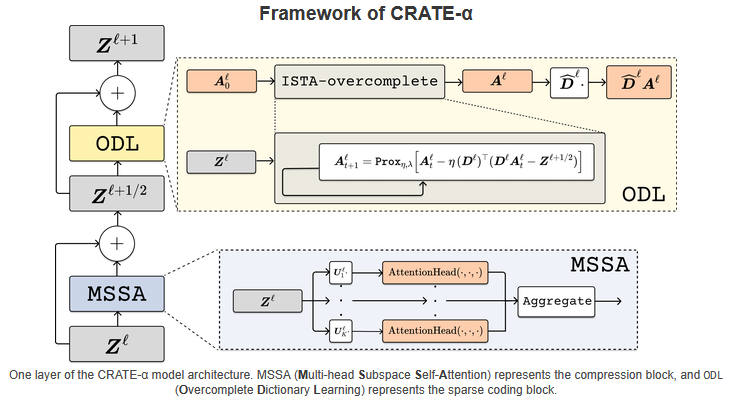
\includegraphics[width=\linewidth]{attachments/crate_alpha_framework.png}
    \caption{One layer of the CRATE-$\alpha$ architecture: MSSA (compression block) followed by ODL (sparse coding block, unrolled as ISTA-overcomplete).}
    \label{fig:crate-alpha-framework}
\end{figure}

\begin{figure}[ht]
    \centering
    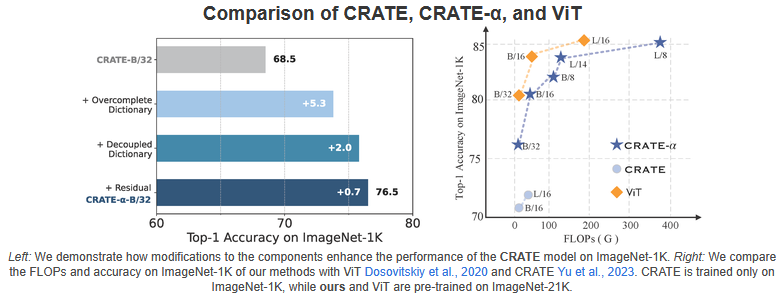
\includegraphics[width=\linewidth]{attachments/crate_alpha_ablation_scaling.png}
    \caption{Left: ablation of CRATE-$\alpha$'s modifications on ImageNet-1K top-1 accuracy. Right: accuracy vs.\ FLOPs comparison of CRATE, CRATE-$\alpha$, and ViT.}
    \label{fig:crate-alpha-scaling}
\end{figure}

\begin{figure}[ht]
    \centering
    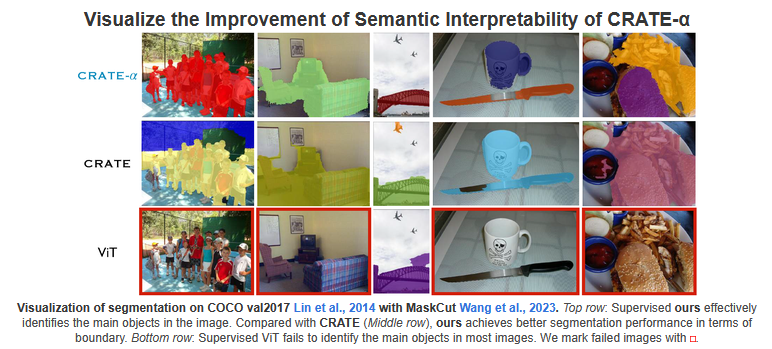
\includegraphics[width=\linewidth]{attachments/crate_alpha_interpretability.png}
    \caption{Segmentation via attention maps on COCO val2017: CRATE-$\alpha$ (top) and CRATE (middle) localize objects more cleanly than a supervised ViT (bottom, failures marked in red).}
    \label{fig:crate-alpha-interpretability}
\end{figure}

\section{Proposed Implementation Strategy}

\subsection{Phase 1: LISTA Baseline Setup}
The immediate next step is implementing standard LISTA (Section~I.A) on synthetic sparse-signal data in PyTorch: a fixed random measurement matrix $A$, artificially generated sparse ground-truth signals $x^{\text{true}}$, and simulated noisy measurements $b = Ax^{\text{true}} + n$. This baseline serves two purposes: it validates the mathematical derivation worked through in this report against an actual trained model, and it establishes a reusable training pipeline (dataset generation, forward pass, backpropagation through unrolled layers) for whatever comes next. Target: NMSE benchmarking against classical ISTA, replicating the qualitative convergence-speed gap shown in Fig.~3.

\subsection{Phase 1: LISTA Baseline Results}
This baseline has been implemented and trained. Using a fixed random Gaussian measurement matrix $A \in \mathbb{R}^{250 \times 500}$, sparse ground-truth signals $x^{\text{true}}$ with 10\% support density, and additive noise ($\sigma = 0.01$) forming simulated measurements $b = Ax^{\text{true}} + n$, a $K=16$-layer LISTA network with fully untied parameters ($W_1^k, W_2^k, \theta^k$ free at every layer) was trained via Adam on synthetic $(x^{\text{true}}, b)$ pairs, minimizing the standard MSE loss.

On a held-out test batch, the trained network reaches \textbf{-11.16 dB NMSE} at $k=16$ layers. Classical ISTA, run to convergence at three fixed step sizes, requires \textbf{79 iterations} ($\lambda = 0.1$) to \textbf{269 iterations} ($\lambda = 0.025$) to reach that same NMSE — a roughly \textbf{5--17$\times$} reduction in iterations/layers for LISTA to match ISTA's accuracy (Fig.~\ref{fig:lista-vs-ista-results}). This qualitatively reproduces the LISTA-over-ISTA convergence-speed gap described in Section~I.A.3, though at a smaller magnitude than the $\sim$50$\times$ figure reported in the literature (Gregor and LeCun, 2010) — consistent with the reduced problem scale ($250\times500$ vs.\ the larger dictionaries used in published benchmarks) and limited training budget (2{,}000 epochs, single random seed) of this initial run. This establishes a working, reusable training pipeline (dataset generation, forward pass, backpropagation through unrolled layers) for Phase 2.

\begin{figure}[ht]
    \centering
    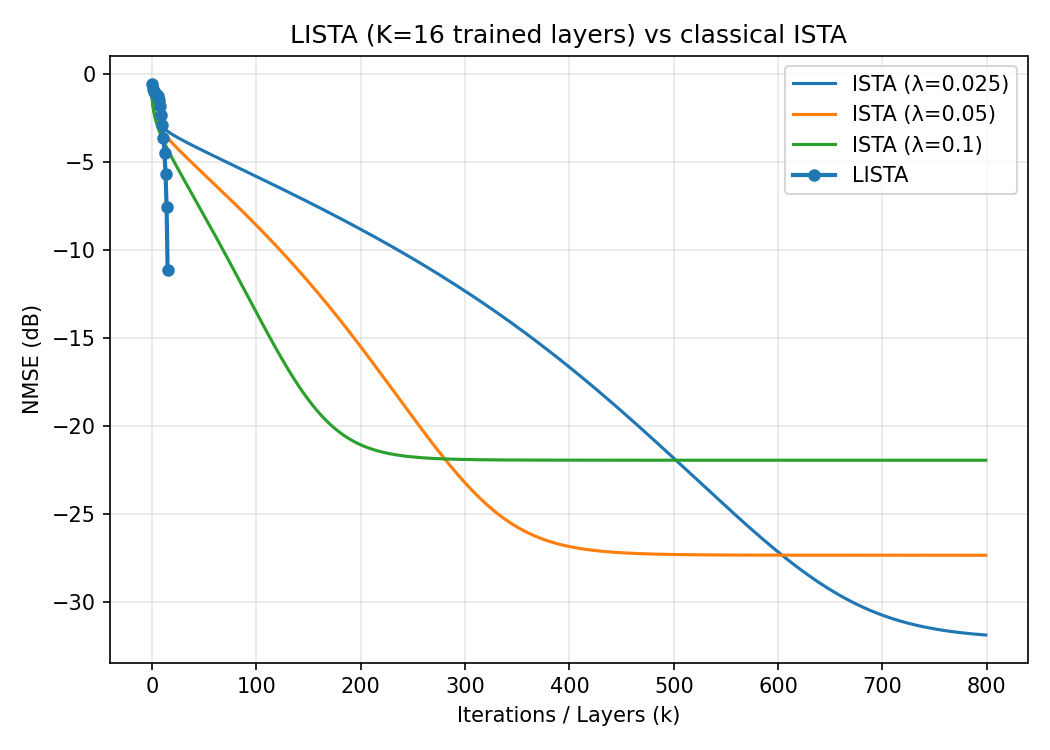
\includegraphics[width=\linewidth]{attachments/lista_vs_ista_nmse.png}
    \caption{NMSE (dB) vs.\ iterations/layers: trained LISTA ($K=16$, untied) vs.\ classical ISTA at three fixed $\lambda$ values, on synthetic sparse-recovery data. Reproduces the qualitative convergence-speed gap of Fig.~3 at smaller scale.}
    \label{fig:lista-vs-ista-results}
\end{figure}

\subsection{Phase 2: CRATE Verification}
Phase 2 implements a small-scale CRATE model (a handful of MSSA + ODL layers, per Fig.~\ref{fig:crate-alpha-framework}) trained on CIFAR-10, using the authors' open-source implementation (Ma-Lab-Berkeley/CRATE) as reference. This phase is explicitly a mechanics-verification exercise rather than a research contribution: the goal is to confirm, hands-on, that the compression (MSSA) and sparsification (ODL) sub-steps behave as an unrolled two-part iteration the way LISTA's gradient and soft-thresholding steps do, and to build working familiarity with the architecture before attempting any domain-specific extension of it.

\textbf{Decision point:} Phase 2 begins once Phase 1's baseline reproduces the expected LISTA convergence behavior against classical ISTA. If that validation proves harder than expected, Phase 2 is scoped down to verifying a single CRATE layer's forward-pass mechanics numerically, rather than a full trained model.

\subsection{Phase 3 (Contingent): A Signal-Processing-Specific White-Box Transformer}
Recent work has extended the CRATE framework beyond vision \cite{huang2026prism} by re-deriving its unrolled compression/sparsification steps from a domain-specific physical forward model rather than a generic token-compression objective — for instance, extending the sparse rate reduction derivation to complex-valued RF signals, or unfolding a structured low-rank model of MRI k-space into an attention-like layer. A natural third phase, contingent on identifying a suitable forward model would follow the same pattern for a signal of interest: deriving what an MSSA/ODL-equivalent pair of unrolled steps would look like for that signal's specific measurement model, rather than reusing the generic image-token version verified in Phase 2. This phase is not yet scoped and depends on Phase 2's outcome and advisor input on a concrete target signal/problem.

\section{Future Work}
Beyond the implementation plan in Section~IV, several directions are being weighed as potential candidates for the project's primary novel contribution.

\subsection{Unrolling with Diffusion-Model Priors}
Recent work combines classical unrolling and plug-and-play schemes with diffusion models as learned priors:
\begin{itemize}
    \item[\textbullet] \textit{Mechanism:} Replaces the fixed denoiser or CNN step in architectures like DUBLID or ADMM-CSNet (Sections~I.E, I.E.3) with a pretrained diffusion model (e.g., DMPlug, NeurIPS 2024 \cite{wang2024dmplug}; SILO, 2025 \cite{raphaeli2025silo}).
    \item[\textbullet] \textit{Relevance:} Directly extends the inverse-problem material developed in this report and represents an active, empirically strong direction in the unrolling literature with an established publication record.
\end{itemize}

\subsection{A CRATE-Based Extension}
Building upon CRATE and CRATE-$\alpha$ (Section~III), which derive a white-box Transformer by unrolling the sparse rate reduction objective:
\begin{itemize}
    \item[\textbullet] \textit{Scope:} Beyond the mechanics-verification exercise in Section~IV (Phase~2), this direction aims to derive an analogous unrolled compression/sparsification pair for a different signal or objective, rather than reusing the generic image-token formulation.
    \item[\textbullet] \textit{Trade-offs:} Represents a higher-risk, higher-reach direction given the required mathematical derivations and the rapid pace of current white-box Transformer research.
\end{itemize}

\subsection{Uncertainty-Aware Unrolling}
Extending the EKF and KalmanNet material developed in Section~I.E.7 to produce calibrated uncertainty alongside point estimates:
\begin{itemize}
    \item[\textbullet] \textit{Approach:} Existing variants such as Cholesky-KalmanNet \cite{ko2024cholesky} modify the network to preserve a valid error-covariance structure.
    \item[\textbullet] \textit{Open Gap:} General, well-calibrated uncertainty quantification for unrolled architectures remains largely unresolved.
\end{itemize}

\subsection{Mitigating the Curse of Unrolling: Gradient Instability}
A primary theoretical bottleneck in deep algorithm unrolling is gradient instability—exploding or vanishing gradients that worsen with depth during backpropagation through many unrolled optimization steps \cite{chen2022curse, mehmood2026curse, gao2025learning}:
\begin{itemize}
    \item[\textbullet] \textit{Solution Path:} Stability-inducing unrolling techniques and self-supervised frameworks such as Self-STORM \cite{maj2022combining, sahel2024selfstorm} serve as key starting points to mitigate this instability without relying on massive supervised datasets.
\end{itemize}

\subsection{Unrolling for Graph Signals}
Algorithm unrolling has seen limited but growing application to graph-structured data:
\begin{itemize}
    \item[\textbullet] \textit{Applications:} Focuses on graph topology inference, source localization, and graph signal denoising, with adaptations to learned graph node embeddings appearing as recently as 2024 \cite{shlezinger2025deep}.
    \item[\textbullet] \textit{Considerations:} Represents a cold-start direction due to the required Graph Signal Processing (GSP) background, but addresses a notable open gap in the literature.
\end{itemize}

\subsection{Unrolling Beyond Convex Optimization}
While algorithm unrolling has primarily focused on convex problems (e.g., LASSO, compressive sensing):
\begin{itemize}
    \item[\textbullet] \textit{Long-Horizon Goal:} Extension to non-convex and combinatorial optimization remains largely open. This serves as a long-term theoretical direction rather than a near-term target given the requisite optimization-theory background.
\end{itemize}

\section{Conclusion}
This report worked through algorithm unrolling from classical optimization theory to interpretable deep learning. By breaking down architectures like LISTA and white-box transformers like CRATE, it highlights how embedding mathematical priors directly into network layers bridges the gap between theoretical reliability and computational efficiency. The initial PyTorch implementation validated this practically, demonstrating that a learned solver can hit classical accuracy benchmarks in a fraction of the typical iterations. With the foundational theory and mathematical prerequisites now established, the project can pivot from replication to active exploration. Phase 2 (CRATE verification) is the immediate next step, with Phase 3 and the Future Work directions in Section V contingent on those initial results.
\nocite{*}
\bibliographystyle{IEEEtran}
\bibliography{references} 
% Add Monga et al. (2020) and Gregor & LeCun (2010) to your .bib file

\end{document}